\documentclass[10pt,a4paper]{report}
\usepackage[left=3.00cm, right=1.00cm, top=2.00cm, bottom=2.00cm, nohead, footskip=7mm]{geometry}
\usepackage[14pt]{extsizes}

\usepackage[utf8]{inputenc}
\usepackage[T1]{fontenc}
\usepackage{amsmath}
\usepackage{amsfonts}
\usepackage{amssymb}
\usepackage{pdfpages}
\usepackage{longtable}

\usepackage[russian]{babel}

% Ссылки внутри текста
\usepackage{hyperref}

% Отступ абзаца
\usepackage{indentfirst}
\setlength{\parindent}{1.5cm} 

% Межстрочный интервал
\usepackage{setspace}
\onehalfspacing % интервал 1.5

% Вставка изображений
\usepackage{graphicx}
\graphicspath{{../pic/}}
\RequirePackage{caption}
\DeclareCaptionLabelSeparator{defffis}{ --- }
\captionsetup{justification=centering,labelsep=defffis}

% Настройка оглавлений
\usepackage{titlesec}
\newcommand{\hsp}{\hspace{20pt}}
\titleformat{\chapter}[hang]{\large\bfseries}{\thechapter{. }}{0pt}{\large\bfseries}
\titlelabel{hlabel-formati}
\titlespacing{\chapter}{42pt}{-80pt}{12pt}
\titleformat{\section}[hang]{\large\bfseries}{\thesection{. }}{0pt}{\large\bfseries}
\titlespacing{\section}{42pt}{12pt}{5pt plus 5pt}
\titleformat{\subsection}[hang]{\large\bfseries}{\thesubsection{. }}{0pt}{\large\bfseries}
\titlespacing{\subsection}{42pt}{12pt}{5pt plus 5pt}


% Настройка списков
\usepackage{enumitem}
\setlist{nolistsep, itemsep=0.3cm,parsep=0pt,leftmargin=1.9cm}

% Настройка листингов
\usepackage{listings}
\lstset{
	language = [Sharp]C,
	extendedchars=\true,
	keepspaces=true,
	basicstyle=\small\sffamily,
	showstringspaces=\false,
	numbers=left,
	stepnumber=1,
	numbersep=5pt,
	frame=single,
	tabsize=2,
	captionpos=t,
	breaklines=true,
	breakatwhitespace=false,
	escapeinside={\#*}{*)}
}



\begin{document}
	\renewcommand\bibname{Список литературы}
	
	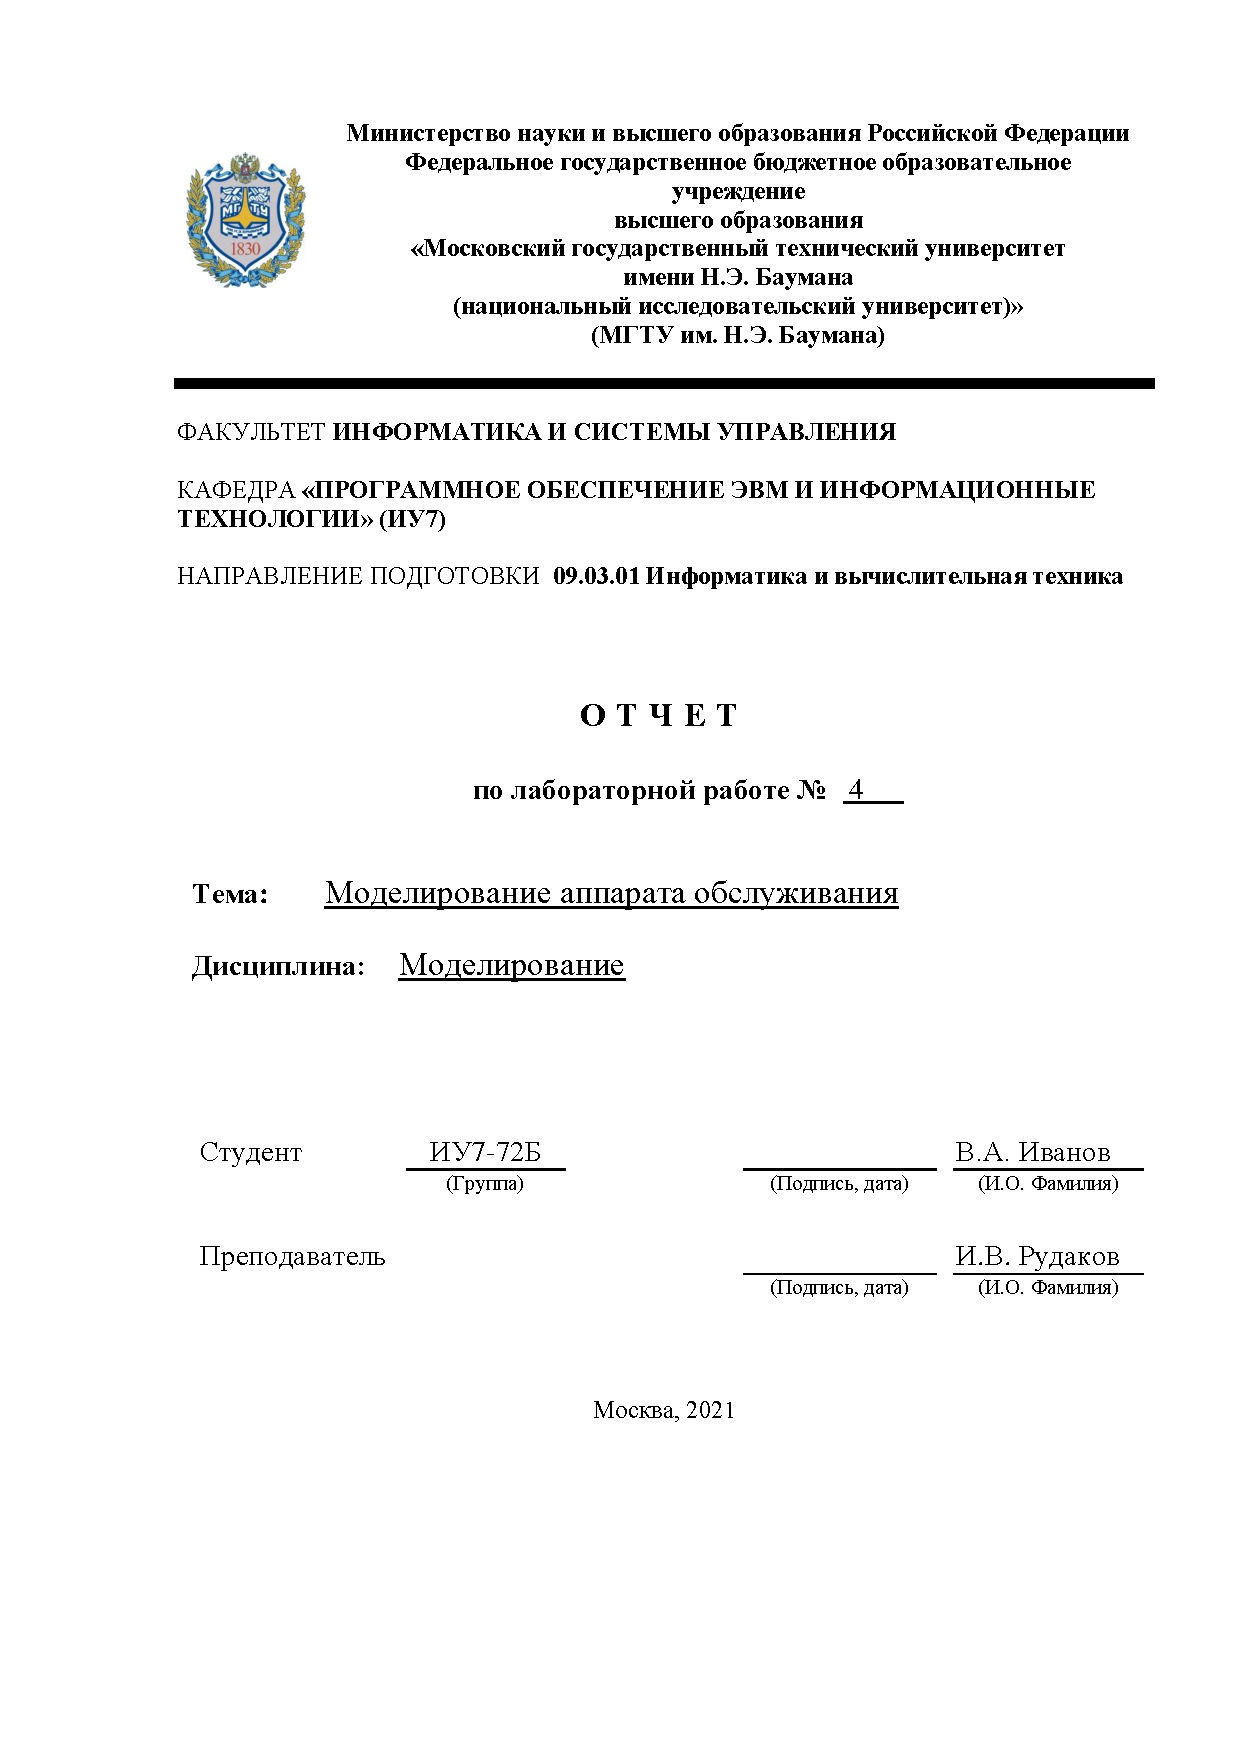
\includepdf[pages=1]{title.pdf}
	
	\chapter{Задание}
	Промоделировать систему, состоящую из генератора, очереди и обслуживающего автомата. Генератор создаёт сообщения по равномерному закону, откуда они поступают в очередь. Из очереди сообщения получает обслуживающий автомат, работающий по закону из первой лабораторной работы (нормальный закон). Определить длину очереди, при которой не произойдёт потери сообщений. Промоделировать двумя методами: пошаговый и событийный.
	
	\chapter{Результаты}
	Примеры построения графиков равномерного и нормального распределения приведены на рисунках \ref{pic:eval} и \ref{pic:norm}.

\begin{figure}[h]
	\begin{center}
		{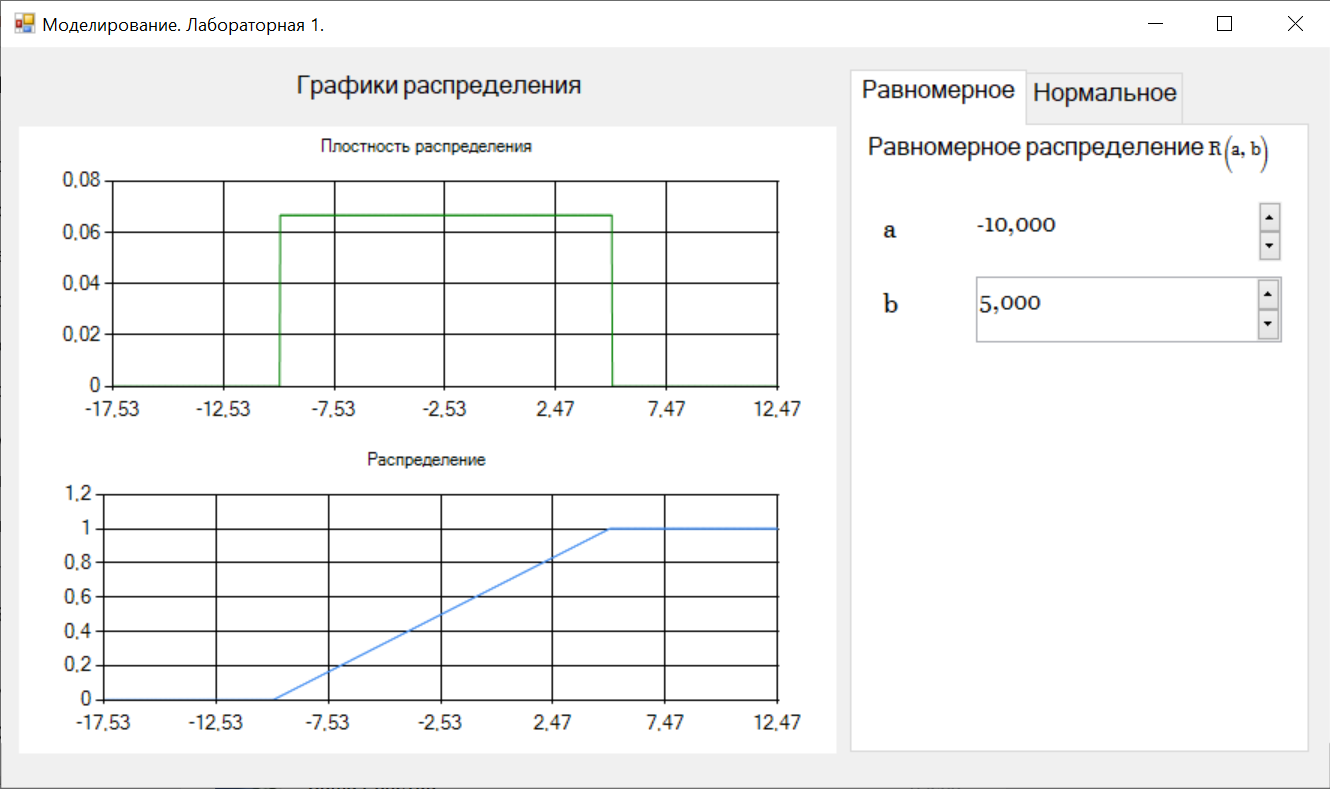
\includegraphics[scale=0.7]{EvalDist}}
		\caption{Графики распределения и плотности распределения для равномерного распределения}
		\label{pic:eval}
	\end{center}
\end{figure}

\begin{figure}[h]
	\begin{center}
		{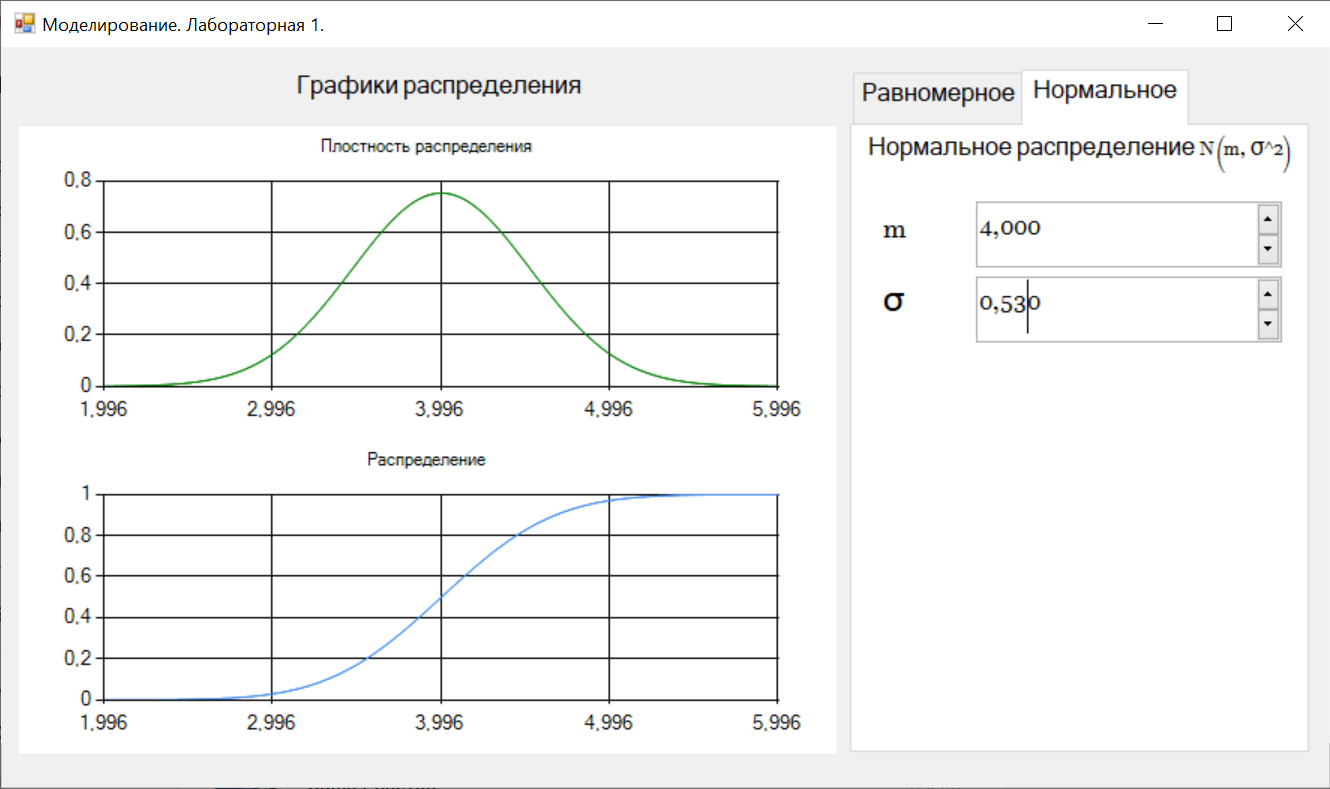
\includegraphics[scale=0.7]{NormDist}}
		\caption{Графики распределения и плотности распределения для нормального распределения}
		\label{pic:norm}
	\end{center}
\end{figure}
	
	\chapter{Текст программы}
	В листинге \ref{lst:prog} представлен фрагмент кода программы, отвечающий за моделирование.

\begin{lstlisting}[caption = {Реализация модели}, label=lst:prog]
public enum EventTypes
{
	NewStudent,
	Lab1Done,
	Lab2Done,
	ExamDone,
	End
}

public abstract class Event : IComparable<Event>
{
	public static Random rnd = new Random();
	public EventTypes type;
	public double time;
	public Event(EventTypes type_, double t_)
	{
		this.type = type_;
		this.time = t_;
	}
	
	public int CompareTo(Event other)
	{
		if (this.time > other.time)
		return 1;
		else
		return -1;
	}
	
	abstract public void Handle(EventModel model);
}

public class EGenerated : Event
{
	public EGenerated(double t_) : base(EventTypes.NewStudent, t_) { }
	public override void Handle(EventModel model)
	{
		Request req = model.Gen.New(model.CurT);
		model.createdN++;
		if (model.createdN < model.maxCreatedN)
		model.AddEvent(new EGenerated(model.Gen.WhenReady()));
		
		var switchOption = rnd.Next() % 3;
		switch (switchOption)
		{
			case 0:
			// Student goes to lab 1
			model.Queues[0].Push(req, model.CurT);
			if (model.Masters[0].IsFree())
			model.AddEvent(new ELab1Done(model.CurT));
			break;
			
			case 1:
			// Student goes to lab 2
			model.Queues[1].Push(req, model.CurT);
			if (model.Masters[1].IsFree() && model.Masters[2].IsFree())
			model.AddEvent(new ELab2Done(model.CurT, 1 + rnd.Next() % 2));
			else if (model.Masters[1].IsFree())
			model.AddEvent(new ELab2Done(model.CurT, 1));
			else if (model.Masters[2].IsFree())
			model.AddEvent(new ELab2Done(model.CurT, 2));
			break;
			
			case 2:
			// Student goes to exam
			model.Queues[2].Push(req, model.CurT);
			if (model.Lecturer.IsFree())
			model.AddEvent(new EExamDone(model.CurT));
			break;
			
			default:
			break;
		}
	}
}

public class ELab1Done : Event
{
	public ELab1Done(double t_) : base(EventTypes.Lab1Done, t_) {}
	
	public override void Handle(EventModel model)
	{
		Request req = model.Masters[0].Get();
		if (req != null)
		{
			if (rnd.NextDouble() < model.Masters[0].ReturnP)
			model.Queues[0].Push(req, model.CurT);
			else
			{
				model.Queues[1].Push(req, model.CurT);
				if (model.Masters[1].IsFree() && model.Masters[2].IsFree())
				model.AddEvent(new ELab2Done(model.CurT, 1 + rnd.Next() % 2));
				else if (model.Masters[1].IsFree())
				model.AddEvent(new ELab2Done(model.CurT, 1));
				else if (model.Masters[2].IsFree())
				model.AddEvent(new ELab2Done(model.CurT, 2));
			}
		}
		
		if (model.Queues[0].Count == 0)
		return;
		req = model.Queues[0].Pop();
		if (req != null)
		{
			model.Masters[0].Put(req, model.CurT);
			model.AddEvent(new ELab1Done(model.Masters[0].WhenReady()));
		}
	}
}

public class ELab2Done : Event
{
	private int Num;
	public ELab2Done(double t_, int num) : base(EventTypes.Lab2Done, t_) {Num = num;}
	
	public override void Handle(EventModel model)
	{
		Request req = model.Masters[Num].Get();
		if (req != null)
		{
			if (rnd.NextDouble() < model.Masters[Num].ReturnP)
			model.Queues[1].Push(req, model.CurT);
			else
			{
				model.Queues[2].Push(req, model.CurT);
				if (model.Lecturer.IsFree())
					model.AddEvent(new EExamDone(model.CurT));
			}
		}
		
		if (model.Queues[1].Count == 0)
			return;
		req = model.Queues[1].Pop();
		if (req != null)
		{
			model.Masters[Num].Put(req, model.CurT);
			model.AddEvent(new ELab2Done(model.Masters[Num].WhenReady(), Num));
		}
	}
}

public class EExamDone : Event
{
	public EExamDone(double t_) : base(EventTypes.ExamDone, t_) { }
	public override void Handle(EventModel model)
	{
		Request req = model.Lecturer.Get();
		if (req != null)
		{
			if (rnd.NextDouble() < model.Lecturer.ReturnP)
				model.denyedN++;
			else
				model.servedN++;
		}
		
		if (model.Queues[2].Count == 0)
			return;		
		req = model.Queues[2].Pop();
		if (req != null)
		{
			model.Lecturer.Put(req, model.CurT);
			model.AddEvent(new EExamDone(model.Lecturer.WhenReady()));
		}
	}
}

public class EventModel
{
	public double CurT;
	public Generator Gen;
	public List<Service> Masters;
	public Service Lecturer;
	public List<ReqQueue> Queues;
	
	public int createdN = 0;
	public int servedN = 0;
	public int denyedN = 0;
	public int maxCreatedN = 300;
	private List<Event> Events;
	
	public EventModel(Generator generator, List<Service> masters, Service lecturer)
	{
		Gen = generator;
		Masters = masters;
		Lecturer = lecturer;
	}
	
	private void Reset()
	{
		createdN = 0;
		servedN = 0;
		denyedN = 0;
		CurT = 0;
		Gen.New(CurT);
		Events = new List<Event> {
			new EGenerated(Gen.WhenReady())
		};
		Queues = new List<ReqQueue> { new ReqQueue(), new ReqQueue(), new ReqQueue() };
	}
	
	public ModelingResult Run()
	{
		Reset();
		while (Events.Count > 0)
		{
			Event e = this.Events[0];
			this.Events.RemoveAt(0);
			CurT = e.time;
			e.Handle(this);
		}
		return new ModelingResult(this.servedN, this.denyedN, this.CurT, this.Queues);
	}
	
	public void AddEvent(Event e)
	{
		Events.Add(e);
		Events.Sort();
	}
}
\end{lstlisting}

	
\end{document}